\documentclass[a4]{beamer}
\usepackage{amssymb}
\usepackage{graphicx}
\usepackage{subfigure}
\usepackage{newlfont}
\usepackage{amsmath,amsthm,amsfonts}
%\usepackage{beamerthemesplit}
\usepackage{pgf,pgfarrows,pgfnodes,pgfautomata,pgfheaps,pgfshade}
\usepackage{mathptmx}  % Font Family
\usepackage{helvet}   % Font Family
\usepackage{color}

\mode<presentation> {
 \usetheme{Default} % was Frankfurt
 \useinnertheme{rounded}
 \useoutertheme{infolines}
 \usefonttheme{serif}
 %\usecolortheme{wolverine}
% \usecolortheme{rose}
\usefonttheme{structurebold}
}

\setbeamercovered{dynamic}

\title[MA4413]{Statistics for Computing \\ {\normalsize MA4413 Lecture 4B and 5B}}
\author[Kevin O'Brien]{Kevin O'Brien \\ {\scriptsize Kevin.obrien@ul.ie}}
\date{Autumn Semester 2013}
\institute[Maths \& Stats]{Dept. of Mathematics \& Statistics, \\ University \textit{of} Limerick}

\renewcommand{\arraystretch}{1.5}

\begin{document}
\begin{frame}
\titlepage
\end{frame}

\begin{frame}
\frametitle{Current Status}
\begin{itemize}
\item Mid Term Examination next Monday (Week 5) at 4pm
\item Currently covering Continuous Probability Distributions
\item Lecture notes are out of synch with published class notes (we are about half a lecture ahead)
\item The Exponential distribution will be examinable. (I will confirm that at the end of this lecture)
\item Next Wednesday We will start looking at the Normal Distribution.
\end{itemize}
\end{frame}

\begin{frame}[fragile]
\frametitle{Continuous Distributions}
\begin{itemize}
\item (The Continuous Uniform Distribution, Not examinable)
\item The Exponential Distribution (Examinable for midterm)
\item The Normal Distribution
\item The Standard Normal (Z) Distribution.
\item Applications of Normal Distribution
\end{itemize}
\end{frame}

\begin{frame}[fragile]
\frametitle{Exponential Distribution}
The Exponential Distribution may be used to answer the following questions:
\begin{itemize}
\item How much time will elapse before an earthquake occurs in a given region?
\item How long do we need to wait before a customer enters our shop?
\item How long will it take before a call center receives the next phone call?
\item How long will a piece of machinery work without breaking down?
\end{itemize}
\end{frame}

\begin{frame}[fragile]
\frametitle{Exponential Distribution}

\begin{itemize}
\item All these questions concern the time we need to wait before a given event occurs. If this waiting time is unknown, it is often appropriate to think of it as a random variable having an exponential distribution.
\item Roughly speaking, the time $X$ we need to wait before an event occurs has an exponential distribution if the probability that the event occurs during a certain time interval is proportional to the length of that time interval.

\end{itemize}
\end{frame}

%------------------------------------------------------------------------%
\begin{frame}[fragile]
\frametitle{Probability density function}
The probability density function (PDF) of an exponential distribution is

\[
f(x) = \begin{cases}
\lambda e^{-\lambda x}, & x \ge 0, \\
0, & x < 0.
\end{cases}\]
The parameter $\lambda$  is called \textbf{\emph{rate}} parameter.
\end{frame}

%------------------------------------------------------------------------%
\begin{frame}[fragile]
\frametitle{Cumulative density function}
The cumulative distribution function (CDF) of an exponential distribution is

\[
F(x) = \begin{cases}
1-e^{-\lambda x}, & x \ge 0, \\
0, & x < 0.
\end{cases}\]

\end{frame}

%------------------------------------------------------------------------%
\begin{frame}[fragile]
\frametitle{Expected Value and Variance}
The expected value of an exponential random variable $X$ is:

\[
E[X] = \frac{1}{\lambda}\]
The variance of an exponential random variable $X$ is:

\[
V[X] = \frac{1}{\lambda^2}\]

\end{frame}

%------------------------------------------------------------------------%
\begin{frame}[fragile]
\frametitle{Exponential Distribution: Example}
Assume that the length of a phone call in minutes is an exponential random variable $X$ with parameter
$\lambda = 1/10$. If someone arrives at a phone booth just before you arrive, find the probability that you
will have to wait \begin{itemize}
\item[(a)] less than 5 minutes,
\item[(b)] between 5 and 10 minutes.
\end{itemize}
\end{frame}



%%------------------------------------------------------------------------%
%\begin{frame}[fragile]
%\frametitle{Exponential Distribution: Example}
%\begin{verbatim}
%> dexp(0:10,rate=0.10)
% [1] 0.10000000 0.09048374 0.08187308 0.07408182 0.06703200 0.06065307
% [7] 0.05488116 0.04965853 0.04493290 0.04065697 0.03678794
%>
%> pexp(0:10,rate=0.10)
% [1] 0.00000000 0.09516258 0.18126925 0.25918178 0.32967995 0.39346934
% [7] 0.45118836 0.50341470 0.55067104 0.59343034 0.63212056
%\end{verbatim}
%\end{frame}

%------------------------------------------------------------------------%
\begin{frame}[fragile]
\frametitle{Exponential Distribution: Example}

As it is CDF values that we are interested in, we use the output from the \texttt{pexp()} commands.

\begin{itemize}
\item[(a)] $P(X \leq 5)$ = 0.39346934
\item[(b)] $P(5 \leq X \leq 10)$ \\ = $P( X \leq 10) - P( X \leq 5)$ \\ = 0.63212056- 0.39346934 \\ = 0.2386512 \\= 23.84 $\%$
\end{itemize}

\end{frame}



%------------------------------------------------------------------------%
\begin{frame}[fragile]
\frametitle{Exponential Distribution}
\begin{itemize}
\item The Exponential Rate
\item Related to the Poisson mean (m)
\item If we expect 12 occurrences per hour - what is the rate?
\item We would expected to wait 5 minutes between occurrences.
\end{itemize}
\end{frame}

\end{document}
%------------------------------------------------------------------------%
\begin{frame}
\frametitle{ Today's Class }
\begin{itemize}
\item Continuous Random Variables
\item The Normal Distribution
\item Characteristics of the Normal Distribution
\item The Standard Normal (Z) Distribution
\item Using Murdoch Barnes Table 3
\item Standardization Formula
\item Important Formulae
\end{itemize}
\end{frame}
%------------------------------------------------------------%
\begin{frame}
\frametitle{Continuous Random variables}
\begin{itemize}
\item Previously we have been studying discrete random variables, such as the Binomial and the Poisson random variables.
\item Now we turn our attention to continuous random variables.
\item Recall that a continuous random variable is one which takes an infinite number of possible values, rather than just a countable number of distinct values.
\item Continuous random variables are usually measurements.
\item Examples include height, weight, the amount of sugar in an orange, the time required to run a mile.
\end{itemize}

\end{frame}
%------------------------------------------------------------%
\begin{frame}

\frametitle{Introduction to the Normal Distribution}
\begin{itemize}
\item
Recall the experiment whereby a die was rolled 100 times, and the sum of the 100 values was recorded.
\item
This experiment was repeated a very large number of times (e.g. 100,000 times ) in a simulation study.
\item
A histogram was drawn to depict the distribution of outcomes of this experiment.
\item Recall that we agreed that ``bell-shaped" was a good description of the histogram.

\end{itemize}
\end{frame}


\frame{
\frametitle{Normal Distribution}

\begin{center}
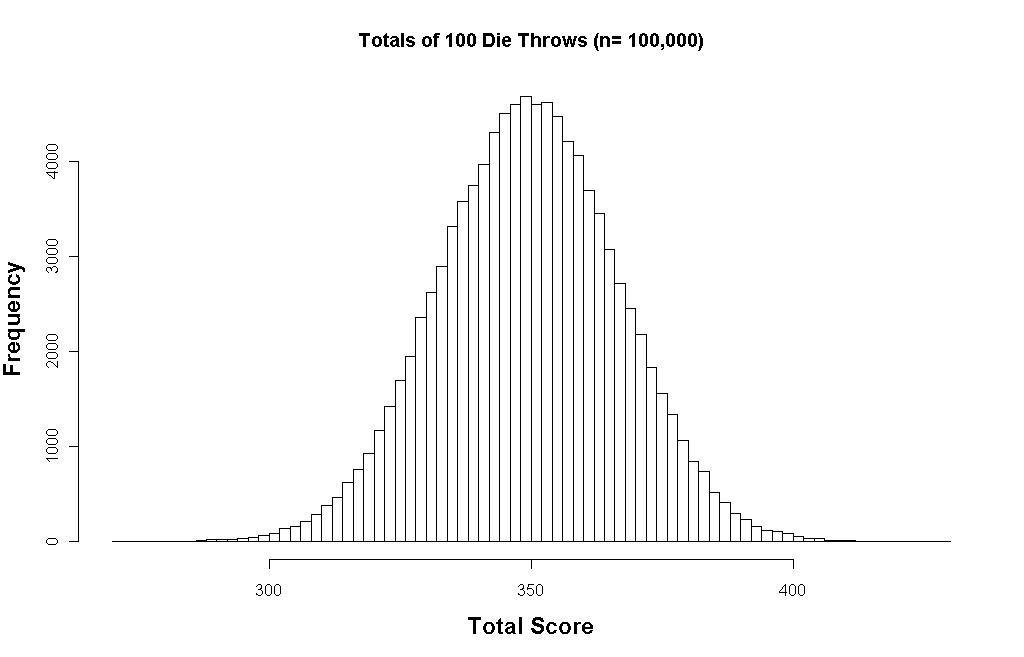
\includegraphics[scale=0.30]{3aDieHist3}
\end{center}

}



\frame{
\frametitle{Normal Distribution}
\begin{itemize}
\item The normal distribution is perhaps the most widely used distribution for a random variable.
\item Normal distributions have the same general shape: the bell curve.
\item They are symmetric with scores more concentrated in the middle than in the tails.
%\item Examples of normal distributions are shown below. Notice that they differ in how spread out they are. The area under each curve is the same.
\item The height of a normal distribution can be defined mathematically in terms of two fundamental parameters: the mean ($\mu$) and the standard deviation ($\sigma$).
\item A normally distributed random variable X is denoted $ X \sim \mbox{N} (\mu, \sigma^2)$ (note that we use the variance term here)
    \item The mean and standard deviation are vital for calculating probabilities.
\end{itemize}
}
%------------------------------------------------------------------------%
\frame{
\frametitle{The Normal Distribution}
The \textbf{\emph{probability density function}} of the normal distribution is given as
\[ f(x) = \frac{1}{\sqrt{2\pi\sigma^2}} e^{ -\frac{(x-\mu)^2}{2\sigma^2} } \]

Integrating this formula would allow us to compute probabilities.
However, we will not use this formula, although we later discuss what a probability density function is.
}

\frame{
\frametitle{Normal Distribution}

\begin{center}
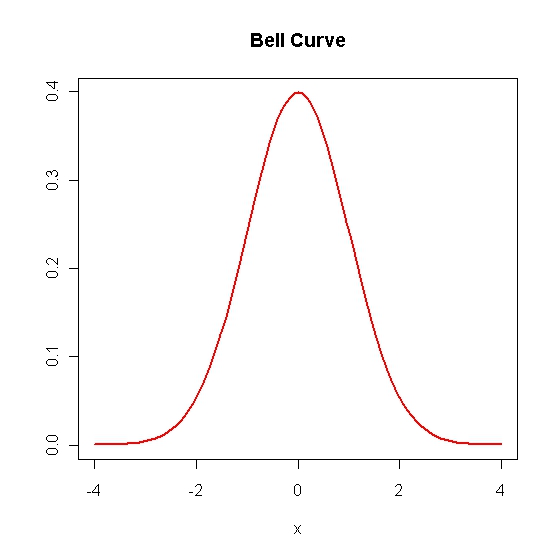
\includegraphics[scale=0.30]{5ABellCurve}
\end{center}

}
%------------------------------------------------------------------%
\frame{
\frametitle{ Characteristics of the Normal probability distribution}
\begin{itemize}
\item[1] The highest point on the normal curve is at the mean, which is also the median and mode of the distribution.
\item[2] \alert{[VERY IMPORTANT]}
The normal probability curve is bell-shaped and symmetric, with the shape of the curve to the left of the mean a mirror image of the shape of the curve to the right of the mean.
\item[3] The standard deviation determines the width of the curve. Larger values of the the standard deviation result in wider flatter curves, showing more dispersion in data.
\item[4] The total area under the curve for the normal probability distribution is 1.
\end{itemize}
}
%------------------------------------------------------------------%
\frame{
\frametitle{ Characteristics of the Normal probability distribution}
\begin{itemize}
\item The interval defined by the mean $ \pm 1 \times $ standard deviation includes approximately $68\%$ of the observations, leaving $16\%$ (approx) in each tail.
\item The interval defined by the mean $ \pm 1.96 \times $ standard deviation includes approximately $95\%$ of the observations, leaving $2.5\%$ (approx) in each tail.
\item The interval defined by the mean $ \pm 2.58 \times $ standard deviation includes approximately $99\%$ of the observations, leaving $0.5\%$ (approx) in each tail.
\end{itemize}
\textbf{Remark:} It is useful to know this numbers, but we will do all calculations from first principles.
}
%------------------------------------------------------------------------%
\frame{
\frametitle{The Standard Normal Distribution}

\begin{itemize}

\item The standard normal distribution is a special case of the normal distribution with a mean $\mu= 0$ and a standard deviation $\sigma =1$.
\item We denote the standard normal random variable as $Z$ rather than $X$.
\item The distribution is well described in statistical tables (i.e. Murdoch Barnes Table 3)
\item Rather than computing probabilities from first principles, which is very difficult, probabilities from distributions other than the Z distribution (e.g. X $\sim$($\mu=100, \sigma =15$)) can be computed using the Z distribution, a much easier approach. (We shall demonstrate how shortly.)
\end{itemize}
}
%------------------------------------------------%
\frame{
\frametitle{Standardization formula}
All normally distributed random variables have corresponding $Z$ values, called Z-scores.\\
\bigskip
For normally distributed random variables, the z-score can be found using the \textbf{\emph{standardization formula}};
\[z_o = { x_o - \mu \over \sigma}\]
where $x_o$ is a score from the original normal (``X") distribution, $\mu$ is the mean of the original normal distribution, and $\sigma$ is the standard deviation of original normal distribution.\\
\bigskip
Therefore $z_o$ is the z-score that corresponds to $x_o$.

\begin{itemize}
\item Terms with subscripts mean particular values, and are not variable names.
\item The z distribution will only be a normal distribution if the original distribution (X) is normal.
\end{itemize}
}

%------------------------------------------------------------------------%
\frame{
\frametitle{The Standardized Value}
\Large
\begin{itemize}
\item Suppose that mean $\mu = 80 $ and that standard deviation $\sigma = 8$.
\item What is the Z-score for $x_o = 100$?
\[
z_{100} = {x_0 - \mu \over \sigma} = {100 - 80 \over 8} = {20 \over 8} = 2.5
\]
\item Therefore $z_{100} = 2.5$
\end{itemize}
}
%------------------------------------------------------------------------%
\frame{
\frametitle{Z scores}
A Z-score always reflects the number of standard deviations above or below the mean a particular score is.
Suppose the scores of a test are normally distributed with a mean of 50 and a standard deviation of 9
For instance, if a person scored a 68 on a test, then they scored 2 standard deviations above the mean.

Converting the test scores to z scores, an X value of 68 would yield:
\[ Z = {68 - 50 \over 9} =2 \]

So, a Z score of 2 means the original score was 2 standard deviations above the mean.
}
%------------------------------------------------------------------------%
%\end{document}
% The standardization formula
% used to find Z values

%

%------------------------------------------------------------------------%
\frame{
\frametitle{The Standard Normal (Z) Distribution Tables}
\begin{itemize}
\item Importantly, probabilities relating to the z distribution are comprehensively tabulated in \textbf{\emph{Murdoch Barnes table 3}}.

\item Given a value of $k$ (with k usually between 0 and 4), the probability of a standard normal "Z" random variable being greater than (or equal to) k $P(Z \geq k)$ is given in Murdoch Barnes table 3 .
\item Other statistical tables can be used, but they may tabulate probabilities in a different way.
\end{itemize}
}

%------------------------------------------------------------------------%
\frame{
\frametitle{An Important Identity}
If two values $z_o$ and $x_o$ are related in the following way, for some values $\mu$ and $\sigma$,
\[
z_{0} = {x_0 - \mu \over \sigma}
\]
Then we can can say

\[ P(X \geq x_o) = P(Z \geq z_o) \]

or alternatively

\[ P(X \leq x_o) = P(Z \leq z_o) \]

This is fundamental to solving problems involving normal distributions.

}

%------------------------------------------------------------------------%
\frame{
\frametitle{Using Murdoch Barnes tables 3}
\begin{itemize}
\item For some value $z_o$, between 0 and 4, the Murdoch Barnes tables set 3 tabulate $P(Z \geq z_o)$
\item Ideally $z_o$ would be specified to 2 decimal places. If it is not, round to the closest value.
\item We call the third digit (i.e. the digit in the second decimal place) the ``second precision".
\end{itemize}
}

%------------------------------------------------------------------------%
\frame{
\frametitle{Using Murdoch Barnes tables 3}
\begin{itemize}
\item To compute the relevant probability we express $z_o$ as the sum of $z_o$ without the second precision, and the second precision.(For example $1.28 = 1.2 + 0.08$.)
\item Select the row that corresponds to $z_o$ without the second precision (e.g. 1.2).
\item Select the column that corresponds to the second precision(e.g. 0.08).
\item The value that contained on the intersection is $P(Z \geq z_o)$
\end{itemize}
}

%------------------------------------------------------------------------%
\frame{
\begin{table}[ht]
\frametitle{Find $ P(Z \geq 1.28)$}
\vspace{-1.5cm}
%\caption{Standard Normal Distribution } % title of Table
\centering % used for centering table
\begin{tabular}{|c|| c c c c c c|} % centered columns (4 columns)
\hline %inserts double horizontal lines
& \ldots & \ldots & 0.006 &0.07&0.08&0.09 \\
%heading
\hline \hline% inserts single horizontal line
\ldots & \ldots & \ldots &\ldots& \ldots &\ldots&\dots \\ % inserting body of the table
1.0 & \ldots & \ldots &0.1446& 0.1423 &0.1401&0.1379 \\ % inserting body of the table
1.1 & \ldots & \ldots&0.1230& 0.1210 &0.1190&0.1170 \\ % inserting body of the table
1.2 & \ldots & \ldots&0.1038 & 0.1020 &\alert{0.1003}&0.0985\\
1.3 & \ldots & \ldots &0.0869& 0.0853 &0.0838&0.0823 \\ % inserting body of the table
\ldots & \ldots &\ldots&\ldots & \ldots &\ldots&\ldots\\
\hline %inserts single line
\end{tabular}
%\label{table:nonlin} % is used to refer this table in the text
\end{table}
}

%------------------------------------------------------------------------%
\frame{
\frametitle{Using Murdoch Barnes tables 3}
\begin{itemize}
\item Find $ P(Z \geq 0.60)$
\item Find $ P(Z \geq 1.64)$
\item Find $ P(Z \geq 1.65)$
\item Estimate $P( Z \geq 1.645)$
\end{itemize}
}

%------------------------------------------------------------------------%
\frame{
\begin{table}[ht]
\frametitle{Find $ P(Z \geq 0.60)$}
\vspace{-1.5cm}
%\caption{Standard Normal Distribution } % title of Table
\centering % used for centering table
\begin{tabular}{|c|| c c c c c c|} % centered columns (4 columns)
\hline %inserts double horizontal lines
& 0.00 & 0.01 & 0.02 &0.03&\ldots&\ldots \\
%heading
\hline \hline% inserts single horizontal line \hline
\ldots & \ldots &\ldots &\ldots& \ldots &\ldots&\ldots \\ % inserting body of the table
0.4 & 0.3446 & 0.3409&0.3372 & 0.3336 &\ldots&\ldots\\
0.5 & 0.3085 & 0.3050 &0.3015& 0.2981 &\ldots&\dots \\ % inserting body of the table
0.6 & \alert{0.2743} & 0.2709&0.2676 & 0.2643 &\ldots&\ldots\\
0.7 & 0.2420 & 0.2389 &0.2358& 0.2327 &\ldots&\dots \\ % inserting body of the table
\ldots & \ldots &\ldots &\ldots& \ldots &\ldots&\ldots \\ % inserting body of the table
\hline %inserts single line
\end{tabular}
%\label{table:nonlin} % is used to refer this table in the text
\end{table}
}

%------------------------------------------------------------------------%
\frame{
\begin{table}[ht]
\frametitle{Find $ P(Z \geq 1.64)$ and $ P(Z \geq 1.65)$}
\vspace{-1.5cm}
%\caption{Standard Normal Distribution } % title of Table
\centering % used for centering table
\begin{tabular}{|c|| c c c c c c|} % centered columns (4 columns)
\hline %inserts double horizontal lines
& \ldots & \ldots & 0.04 & 0.05 &0.06&0.07 \\
%heading
\hline \hline% inserts single horizontal line
\ldots & \ldots &\ldots &\ldots& \ldots &\ldots&\ldots \\ %Checked
1.5 & \ldots & 0.0630&0.0618& 0.0606 &0.0594&\dots \\ % inserting body of the table
1.6 & \ldots &0.0516& \alert{0.0505} & \alert{0.0495} &0.0485&\ldots\\
1.7 & \ldots &0.0418 &0.0409& 0.0401 &0.0392&\dots \\ % inserting body of the table
\ldots & \ldots &\ldots &\ldots& \ldots &\ldots&\ldots \\ %Checked
\hline %inserts single line
\end{tabular}
%\label{table:nonlin} % is used to refer this table in the text
\end{table}
}

%------------------------------------------------------------------------%
\frame{
\frametitle{Using Murdoch Barnes tables 3}
\begin{itemize}
\item $ P(Z \geq 1.64) = 0.505$
\item $ P(Z \geq 1.65) = 0.495$ \bigskip
\item $ P(Z \geq 1.645)$ is approximately the average value of $ P(Z \geq 1.64)$ and $ P(Z \geq 1.65)$.
\item $ P(Z \geq 1.645)$ = (0.0495 + 0.0505)/2 = 0.0500. ( i.e. $5\%$ )
\end{itemize}
}
%------------------------------------------------------------------%
\frame{
\frametitle{Exact Probability}
\large
\alert{Remarks:} This is for continuous distributions only.
\begin{itemize}
\item The probability that a continuous random variable will take an exact value is infinitely small.
We will usually treat it as if it was zero.
\item
When we write probabilities for continuous random variables in mathematical notation, we often retain the equality component (i.e. the "...or equal to..").\\
For example, we would write expressions $P(X \leq 2)$ or $P(X \geq 5)$.
\item
Because the probability of an exact value is almost zero, these two expression are equivalent to $P(X < 2)$
or $P(X > 5)$. \item The complement of $P(X \geq k)$ can be written as $P(X \leq k)$.
\end{itemize}
}


%------------------------------------------------------------------%
\frame{
\frametitle{Complement and Symmetry Rules}

Any normal distribution problem can be solved with some combination of the following rules.
\begin{itemize} \item \textbf{Complement rule} \item Common to all continuous random variables
\[P(Z \geq k) = 1 - P(Z \leq k) \]
Similarly
\[P(X \geq k) = 1 - P(X \leq k) \]
\end{itemize}

\[P(Z \leq 1.28) = 1 - P(Z \geq 1.28)  = 1-0.1003 = 0.8997\]
}

%------------------------------------------------------------------%
\frame{
\frametitle{Complement and Symmetry Rules}
\begin{itemize}
\item \textbf{Symmetry rule}
\item
This rule is based on the property of symmetry mentioned previously.
\item
Only the probabilities corresponding to values between 0 and 4 are tabulated in Murdoch Barnes.
\item
If we have a negative value of k, we can use the symmetry rule.
\end{itemize}
\[P(Z \leq -k) = P(Z \geq k) \]
by extension, we can say
\[P(Z \geq -k) = P(Z \leq k) \]
}
%------------------------------------------------------------------%
\frame{
\frametitle{Example}
Find $P(Z \geq -1.28)$
\textbf{Solution}\\
\begin{itemize}
\item Using the symmetry rule
\[P(Z \geq -1.28) = P(Z \leq 1.28) \]
\item Using the complement rule
\[P(Z \geq -1.28) = 1 - P(Z \geq 1.28) \]
\[P(Z \geq -1.28) = 1 - 0.1003 = 0.8997 \]
\end{itemize}
}
%------------------------------------------------------------------%
\frame{
Find the probability of a ``z" random variable being between -1.8 and 1.96?
i.e. Compute $P(-1.8 \leq Z \leq 1.96)$\\
Solution
\begin{itemize}
\item Consider the complement event of being in this interval: a combination of being too low or too high.
\item
The probability of being too low for this interval is $P(Z \leq -1.80) = 0.0359$ (check)
\item
The probability of being too high for this interval is $P(Z \geq 1.96) = 0.0250$ (check)
\item
Therefore the probability of being \textbf{outside} the interval is 0.0359 + 0.0250 = 0.0609.
\item
Therefore the probability of being \textbf{inside} the interval is 1- 0.0609 = 0.9391
$P(-1.8 \leq Z \leq 1.96) = 0.9391$
\end{itemize}
}





%--------------------------------------------------------------
\begin{frame}
The mean time spent waiting by customers before their queries are dealt with at an information centre is 10 minutes.

The waiting time is normally distributed with a standard deviation of 3 minutes.
\begin{itemize}
\item [i)] What percentage of customers will be waiting longer than 15 minutes

\item [ii)] $90\%$ of customers will be dealt with in at most 12 minutes. Is this statement true or false?
Justify your answer.

\item [iii)] What percentage of customers will wait between 7 and 13 minutes before their query is dealt with?
\end{itemize}
\end{frame}
%---------------------------------------------%
\begin{frame}
\frametitle{Solutions}

Let x be the normal random variable describing waiting times\\
$P(X \geq 15) =?$ \\
\bigskip
     First , we find the z-value that corresponds to x = 15  (remember $\mu=10$ and $\sigma=3$  )\\
\[ z_o = { x_o - \mu \over \sigma }  = { 15 - 10 \over 3 } = 1.666 \]
\begin{itemize}
\item We will use $z_o =1.67$
\item Therefore we can say $P(X \geq 15 ) = P(Z \geq 1.67)$
\item The Murdoch Barnes tables are tabulated to give $P(Z \geq z_o)$ for some value $ z_o$ .
\item We can evaluate $P(Z \geq 1.67)$  as 0.0475.
\item Necessarily $P(X \geq 15) = 0.0475$.
\end{itemize}
\end{frame}
\end{document}
%---------------------------------------------%
\begin{frame}
\frametitle{Solutions}
\begin{itemize}
\item "$90\%$ of customers will be dealt with in at most 12 minutes."
\item To answer this question, we need to know  $P(X\leq 12)$
\item First , we find the z-value that corresponds to x = 12  (remember $\mu=10$ and $\sigma=3$ )
\end{itemize}
\[ z_o = { x_o - \mu \over sigma }  = { 12 - 10 \over 2 } = 0.666 \]

\end{frame}

%---------------------------------------------%
\begin{frame}
\frametitle{Solutions}
\begin{itemize}
\item We will use $z_o =0.67$
\item Therefore we can say $P(X \geq 12 ) = P(Z \geq 0.67)  = 0.2514$
\item Necessarily  $P(X \leq 12 ) = P(Z \leq 0.67) = 0.7486$
\item $74.86\%$ of customers will be dealt with in at most 12 minutes.
\item The statement that $90\%$ will be dealt with in at most 12 minutes is false.
\end{itemize}
\end{frame}
%---------------------------------------------%
\begin{frame}
What percentage will wait between 7 and 13 minutes ?\\

$P(7 \leq X \leq 13)   = ?$

\textbf{Solution:}\\
Compute the probability of being too low, and the probability of being too high for the interval.\\The probability of being inside the interval is the complement of the combination of these events.
\end{frame}
%---------------------------------------------%
\begin{frame}
\frametitle{Solutions}
\textbf{Too high:}\\
$P(X \geq 13) = ?$
\[ z_o  = {13 - 10  \over 3} = 1\]

From tables, $P(Z \geq 1) = 0.1587$. Therefore $P(X \geq 13) = 0.1587$\\ \bigskip
\textbf{Too low:}\\
$P(X \leq 7) = ?$
\[ z_o  = {7 - 10  \over 3} = -1\]
By symmetry, and using tables, $P(X \leq 7) = P(Z \leq -1)= 0.1587$\\ \bigskip
\end{frame}
%---------------------------------------------%
\begin{frame}
\frametitle{Solutions}

\[P(7 \leq X \leq 13)  = 1 - [ P(X \leq 7)  + P(X \geq 13) ] \]

\[P(7 \leq X \leq 13)  =  1 - [0.1587+0.1587] = 0.6826\]

\end{frame}
%---------------------------------------------%
\end{document}                       